\documentclass{anstrans}
%%%%%%%%%%%%%%%%%%%%%%%%%%%%%%%%%%%
\title{Validation of Spent Nuclear Fuel Output by Cyclus, a Fuel Cycle Simulator Code}
\author{Gwendolyn J. Chee, Gyutae Park, and Kathryn D. Huff}

\institute{
Dept. of Nuclear, Plasma and Radiological Engineering, University of Illinois at Urbana-Champaign \\
gchee2@illinois.edu
}

%%%% packages and definitions (optional)
\usepackage{graphicx} % allows inclusion of graphics
\usepackage{booktabs} % nice rules (thick lines) for tables
\usepackage{microtype} % improves typography for PDF
\usepackage{xspace}
\usepackage{tabularx}
\usepackage{subcaption}
\newcommand{\SN}{S$_N$}
\renewcommand{\vec}[1]{\bm{#1}} %vector is bold italic
\newcommand{\vd}{\bm{\cdot}} % slightly bold vector dot
\newcommand{\grad}{\vec{\nabla}} % gradient
\newcommand{\ud}{\mathop{}\!\mathrm{d}} % upright derivative symbol
\newcommand{\Cyclus}{\textsc{Cyclus}\xspace}%
\newcommand{\Cycamore}{\textsc{Cycamore}\xspace}%
\newcolumntype{c}{>{\hsize=.56\hsize}X}
\newcolumntype{b}{>{\hsize=.7\hsize}X}
\newcolumntype{s}{>{\hsize=.74\hsize}X}
\newcolumntype{f}{>{\hsize=.1\hsize}X}
\newcolumntype{a}{>{\hsize=.45\hsize}X}
\usepackage{titlesec}
\titleformat*{\subsection}{\normalfont}

\begin{document}
%%%%%%%%%%%%%%%%%%%%%%%%%%%%%%%%%%%%%%%%%%%%%%%%%%%%%%%%%%%%%%%%%%%%%%%%%%%%%%%%
\section{Introduction}
\Cyclus \cite{huff_fundamentals_2016}, a fuel cycle simulator, was used to run a simulation of the
United States' nuclear fuel cycle from 1967 up till 2013. The \Cyclus spent nuclear fuel (SNF) data was compared to SNF data from the U.S Department of Energy (DOE) sponsored Unified Database (UDB) \cite{Peterson_UNF_2017}. The UDB provides comprehensive and consistent technical data on reactor sites and spent nuclear fuel (SNF) from 1967, the beginning of nuclear reactor operation in the United States, up to the year 2013. By comparing both sets of data, baseline comparison models between \Cyclus simulated results and real world metrics are established. 

%%%%%%%%%%%%%%%%%%%%%%%%%%%%%%%%%%%%%%%%%%%%%%%%%%%%%%%%%%%%%%%%%%%%%%%%%%%%%%%%
\section{Motivation}
The United States is currently considering various fuel cycles and geologic disposal options
\cite{DOE_strategy_2013}. These decisions made will be influenced by key criteria such as thermal load of waste packages and the thermal capacity of the selected geologic host media. Temperature information of the waste packages are dependent on the decay heat contribution from the isotopic composition of spent fuel. Accurate spent fuel isotopic composition data will in turn give accurate thermal load data. Therefore, to use \Cyclus to correctly run simulations of thermal loading a nuclear waste repository, \Cyclus must first give isotopic composition and spent fuel mass that closely replicates reality. 

%%%%%%%%%%%%%%%%%%%%%%%%%%%%%%%%%%%%%%%%%%%%%%%%%%%%%%%%%%%%%%%%%%%%%%%%%%%%%%%%
\section{Methodology}
\subsection{\textit{Generating \Cyclus Simulation and Analysis}}
Published data of the 112 commerical nuclear reactors that have operated since 1967 in the United States was used to create a \Cyclus simulation of the United States Nuclear Fuel Cycle. The reactor deployment data was obtained from the Power Reactor Information System's (PRIS) reactor database \cite{IAEA_PRIS_2017}. The relevant data included: country, reactor unit, type, net capacity (MWe), first grid date and shutdown date. From there, data for reactors in the United States were extracted and used to populate the simulation. The depletion calculations for the nuclear fuel in reactors in the simulation are recipe based, which means that isotopic composition recipes for fresh and spent fuel are used. The recipes are taken from a reference depletion calculation from ORIGEN. The recipe was also used for \cite{Bae_Synergistic_2017 and Wilson_adoption_2009}. 

Jinja2 \cite{Ronacher_Jinja2_2018}, a Python templating language, was then used in Python to render the data into an input file that can be accepted by \Cyclus. The output file produced by \Cyclus was also analyzed using Python. 

%add more assumptions

\subsection{\textit{UDB Data Analysis}}
The UDB data contains SNF information from 1967 up till 2013. The dataset included discharged fuel assembly data from each reactor with specific isotopic concentrations and decay heat for each assembly including the date it was discharged \cite{Peterson_UNF_2017}. The data was imported into Python and processed to be compared with \Cyclus data. All scripts and data used are available in \cite{doi_transition_scenarios}. 
%%%%%%%%%%%%%%%%%%%%%%%%%%%%%%%%%%%%%%%%%%%%%%%%%%%%%%%%%%%%%%%%%%%%%%%%%%%%%%%%
\section{Results and Analysis}
The primary outcome of this validation is to provide comparisons between \Cyclus and UDB data for spent fuel mass and major isotopic contributions to the total spent fuel mass. 

\subsection{\textit{Cumulative Total Spent Fuel Mass Comparison}}
Figure \ref{fig:total_original} shows the cumulative spent fuel mass for both \Cyclus and UDB data from 1967 to 2013. The total spent fuel mass produced by \Cyclus is larger than UDB data before the year 2000. The \Cyclus and UDB total spent fuel mass data diverge after 2000, with UDB being larger. The discrepancies can be attributed to rigidity of \Cyclus simulation input with respect to cycle and refuel time. In \Cyclus, the user specifies constant month integer refuel and cycle times for each reactor. In reality, the cycle and refuel times are varied throughout each reactor's lifetime and may not fall in exactly month length-ed times. In the \Cyclus simulation, the cycle time and refuel time were assumed to be constants of 18 and 1 month respectively.   

\begin{figure}[ht] % replace 't' with 'b' to force it to be on the bottom
	\centering
	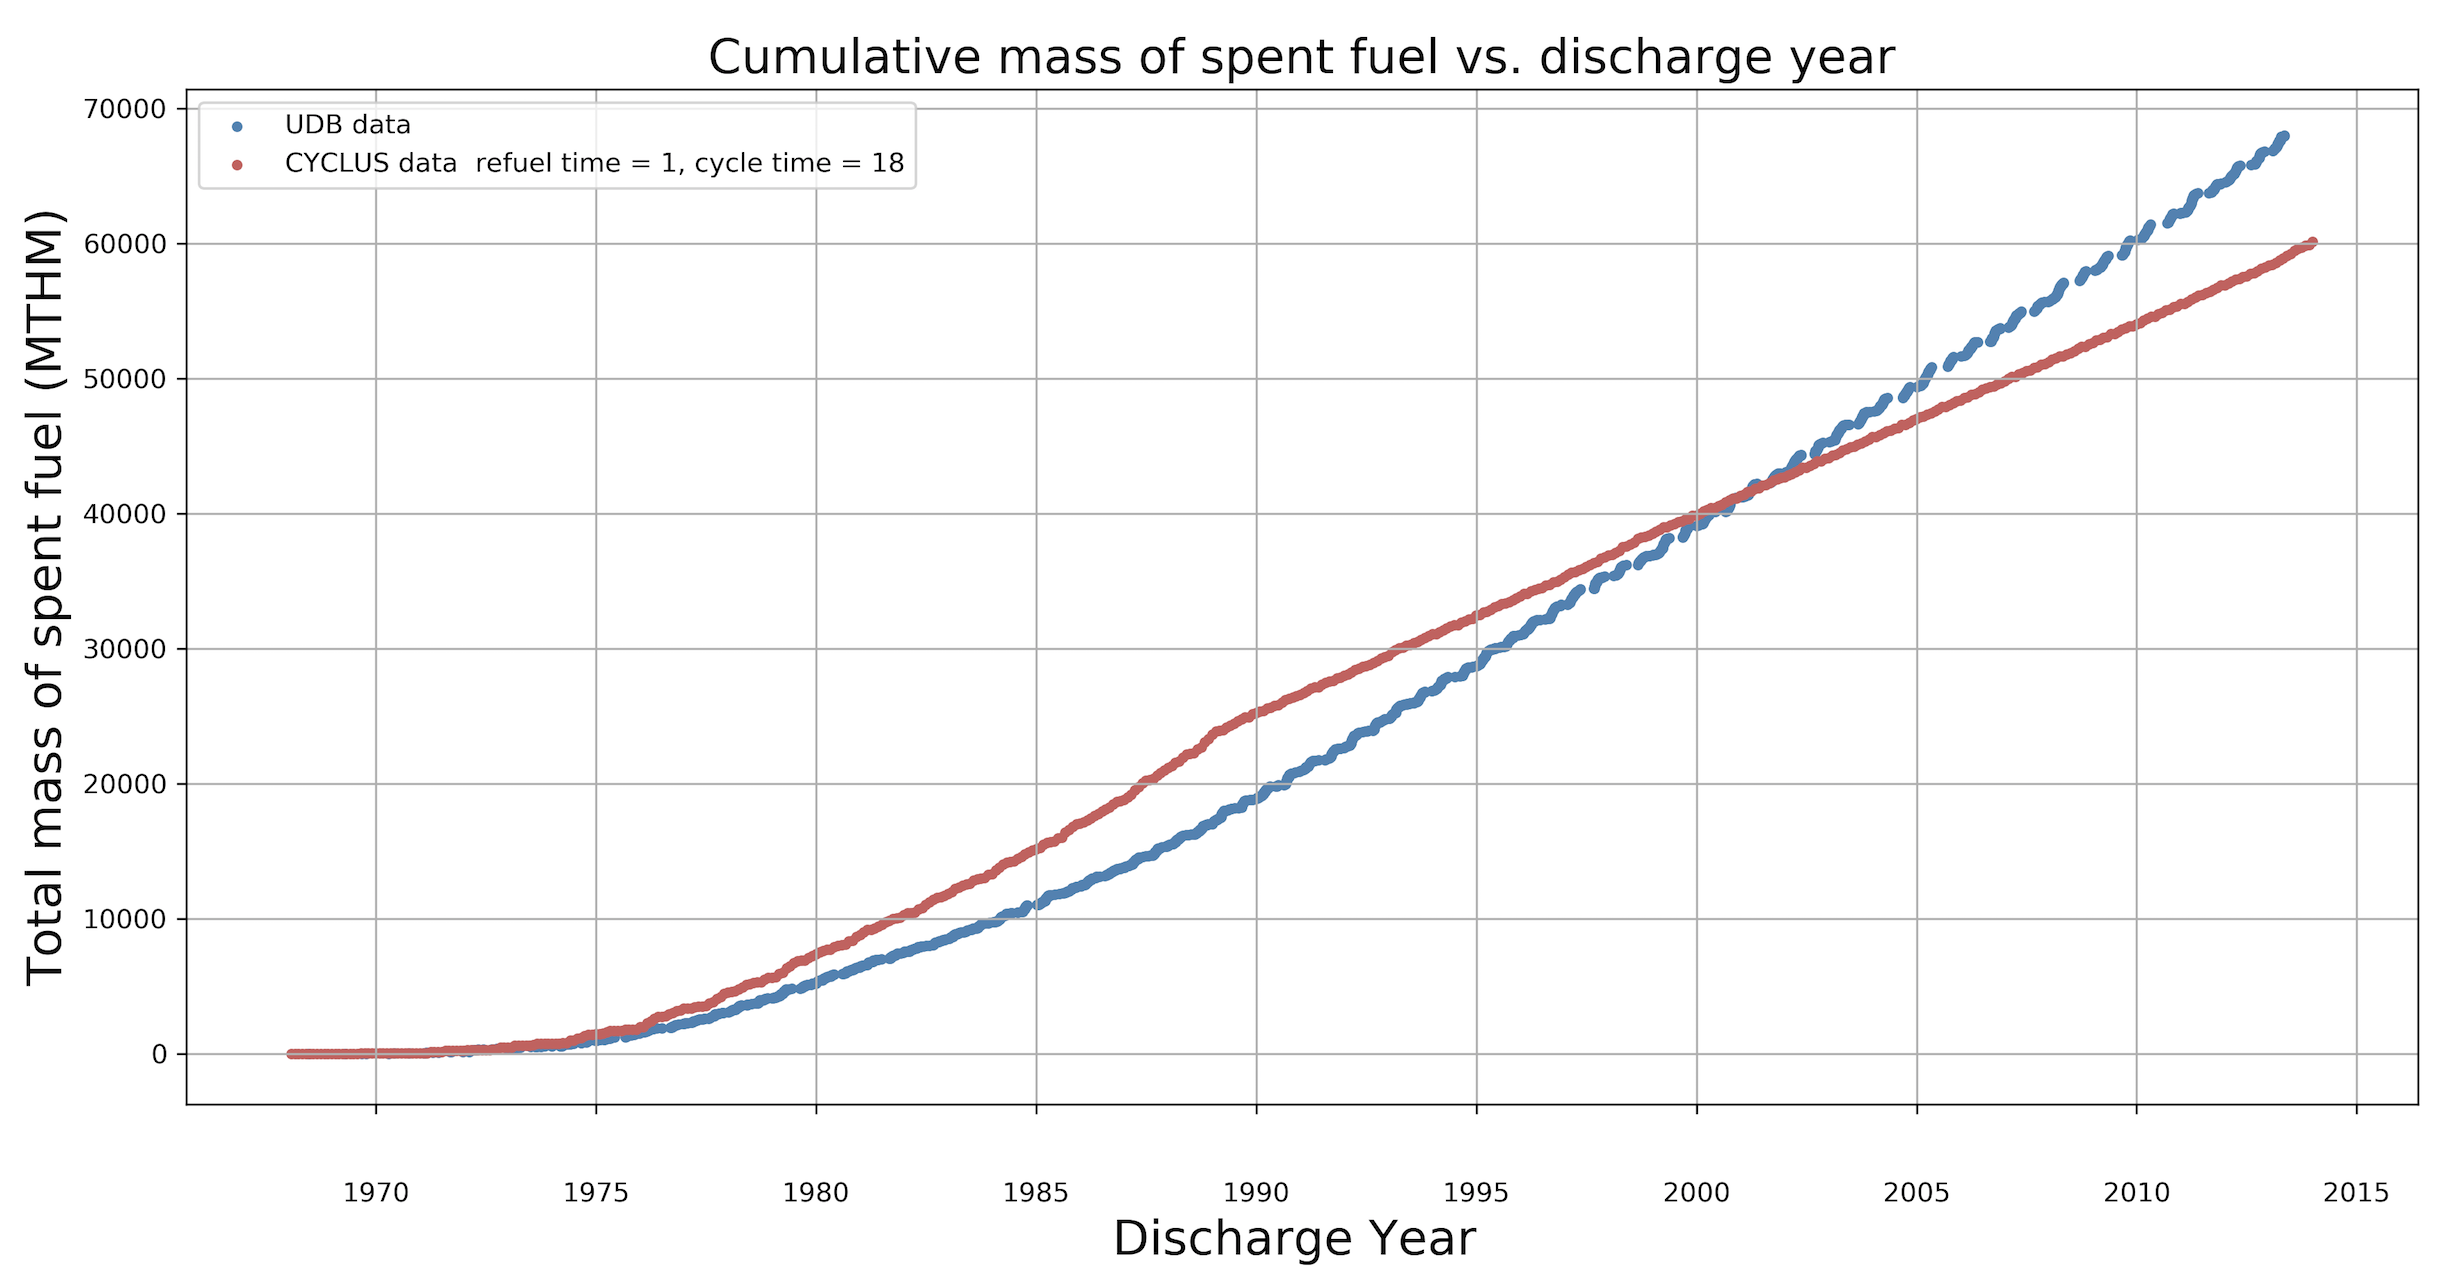
\includegraphics[width=0.48\textwidth]{total_cumulative_mass_spent_fuel_original}
	\caption{Total cumulative spent fuel mass against discharge time for \Cyclus and UDB data from 1967 up to 2013}
	\label{fig:total_original}
\end{figure}

It was reported by the Nuclear Energy Institute (NEI) that there has been significant variance in the refueling period for reactors in the United States. The average refuelling time in 1990 was 104 days, and generally decreased to an average refuelling time of 35 days in 2017 \cite{nei}.

The \Cyclus spent fuel mass data being larger than UDB data before 2000 can be attributed to the assumption that refueling time is always 1 month. Figure \ref{fig:total_refueltime} includes plots of total spent fuel mass from \Cyclus simulations where refuel time is increased. A larger refuel time brings the total spent fuel mass from \Cyclus simulations closer to the UDB data before 2000. 

\begin{figure}[ht] % replace 't' with 'b' to force it to be on the bottom
	\centering
	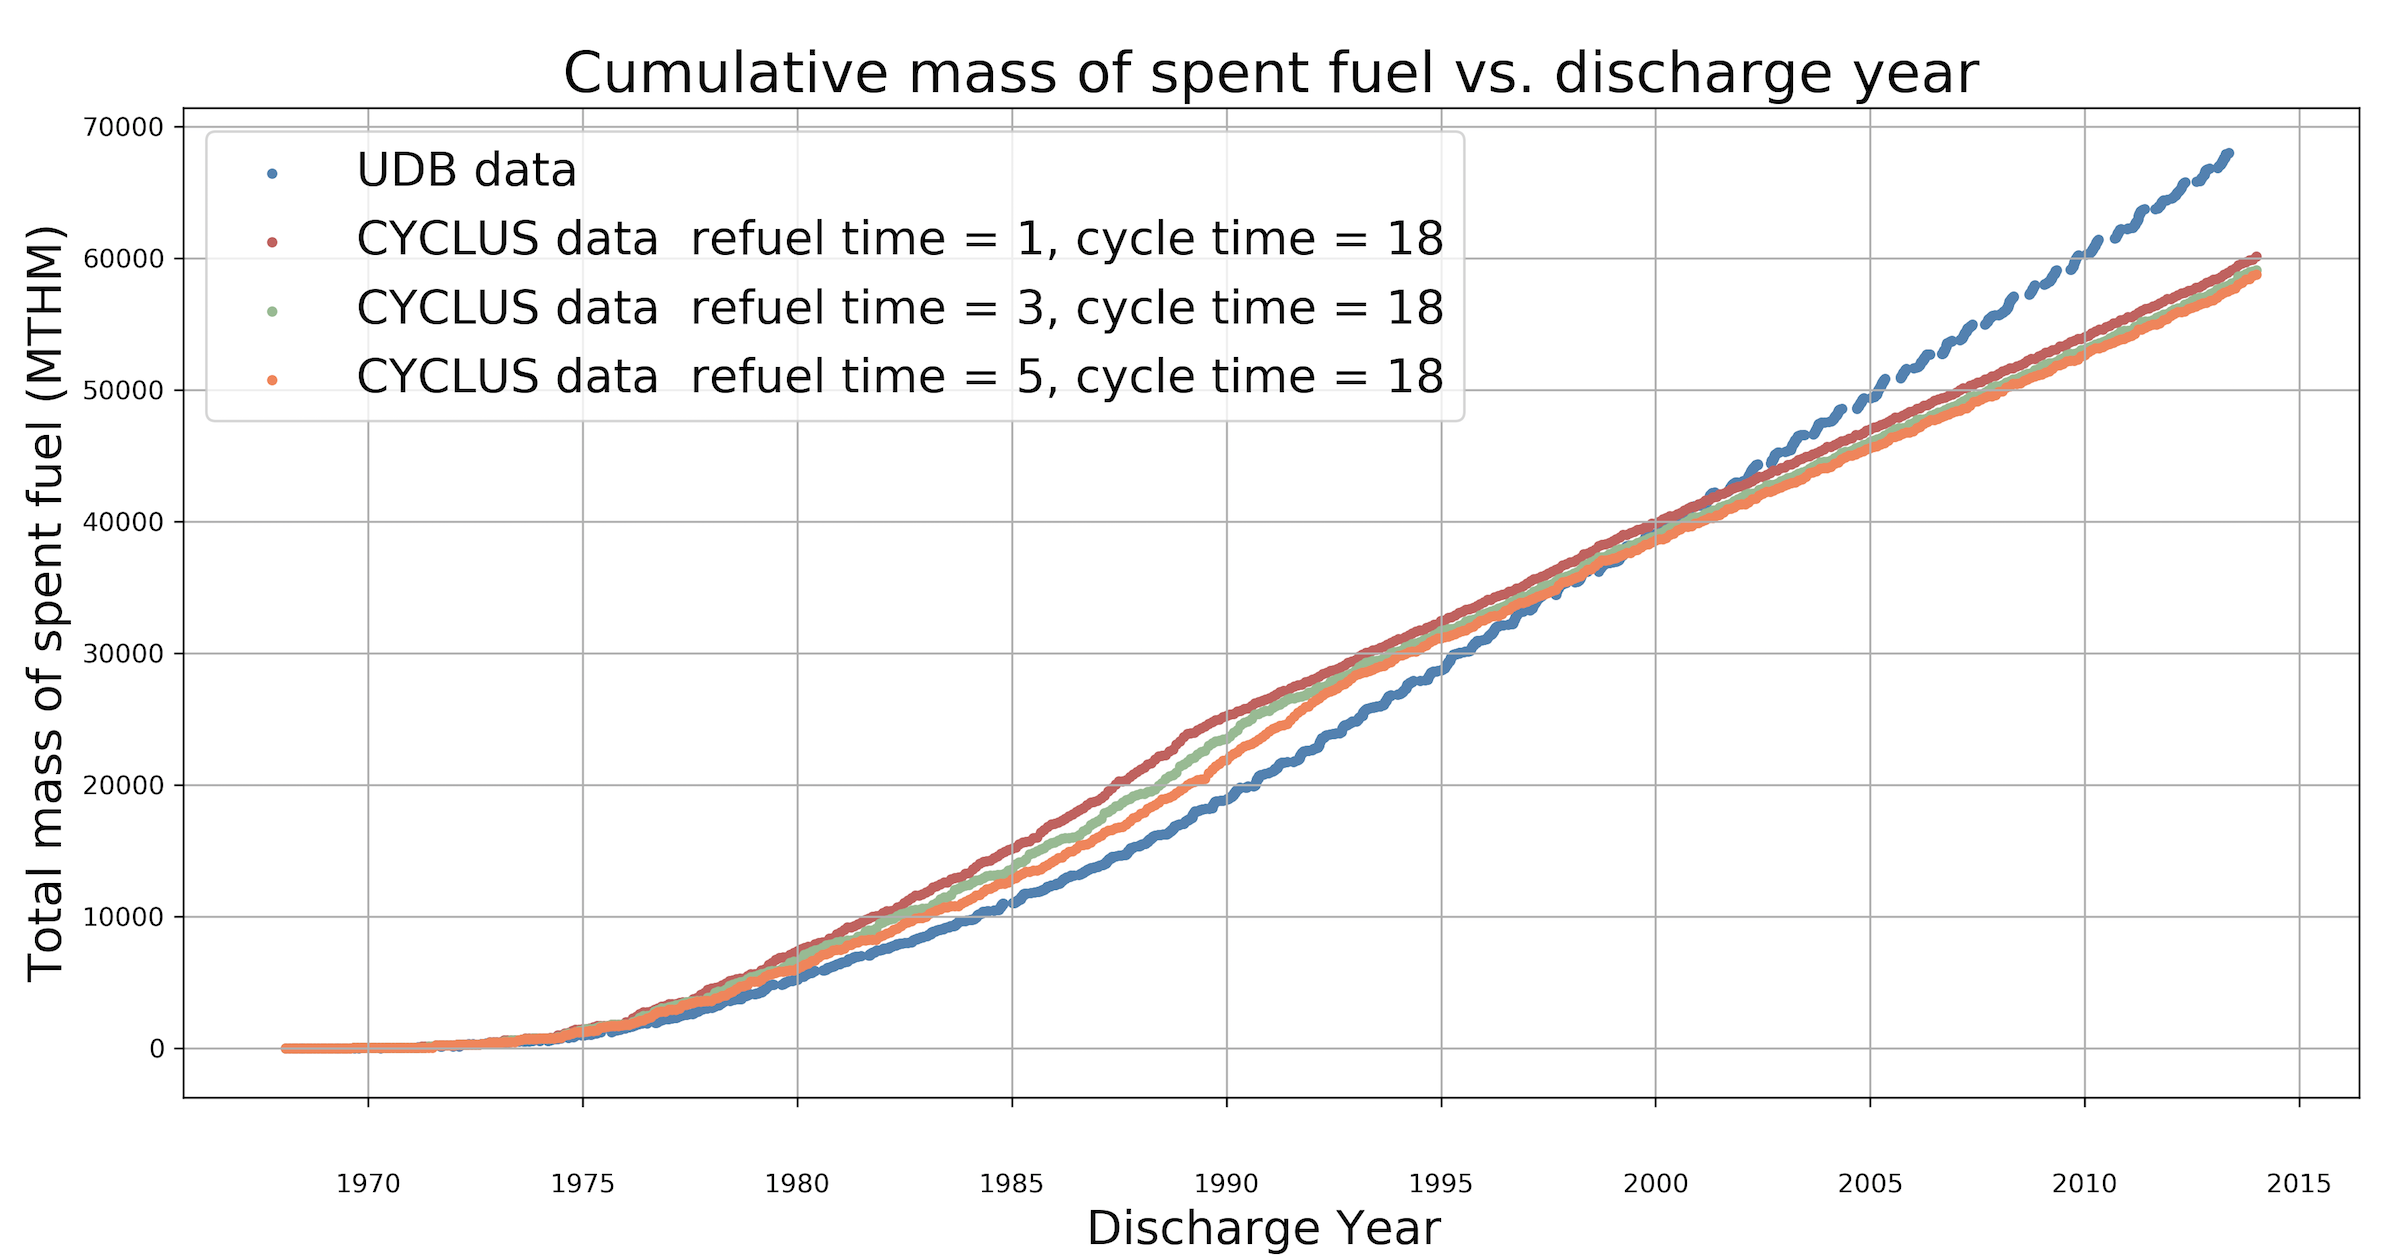
\includegraphics[width=0.48\textwidth]{total_cumulative_mass_spent_fuel_refueltime}
	\caption{Total cumulative spent fuel mass against discharge time for \Cyclus and UDB data from 1967 up to 2013 for varying refuel time}
	\label{fig:total_refueltime}
\end{figure} 

The larger amount of UDB spent fuel mass compared to \Cyclus data after 2000 could be attributed to the cycle length of reality being shorter than the 19 month length of \Cyclus simulations. The United States Department of Energy (DOE) reported that there was a downward trend of forced outage rates of nuclear reactors from 2000 to 2014. The forced outage rate was 4.24\% in 2000 and 2.98\% in 2013. As the rate of forced outages decreased from 2000 to 2013, the cycle length also decreases. 

Figure \ref{fig:total_cycletime} includes plots of total spent fuel mass from \Cyclus simulations where cycle time is varied. A shorter cycle time brings the total spent fuel mass from \Cyclus simulations closer to the UDB data after 2000. 

\begin{figure}[ht] % replace 't' with 'b' to force it to be on the bottom
	\centering
	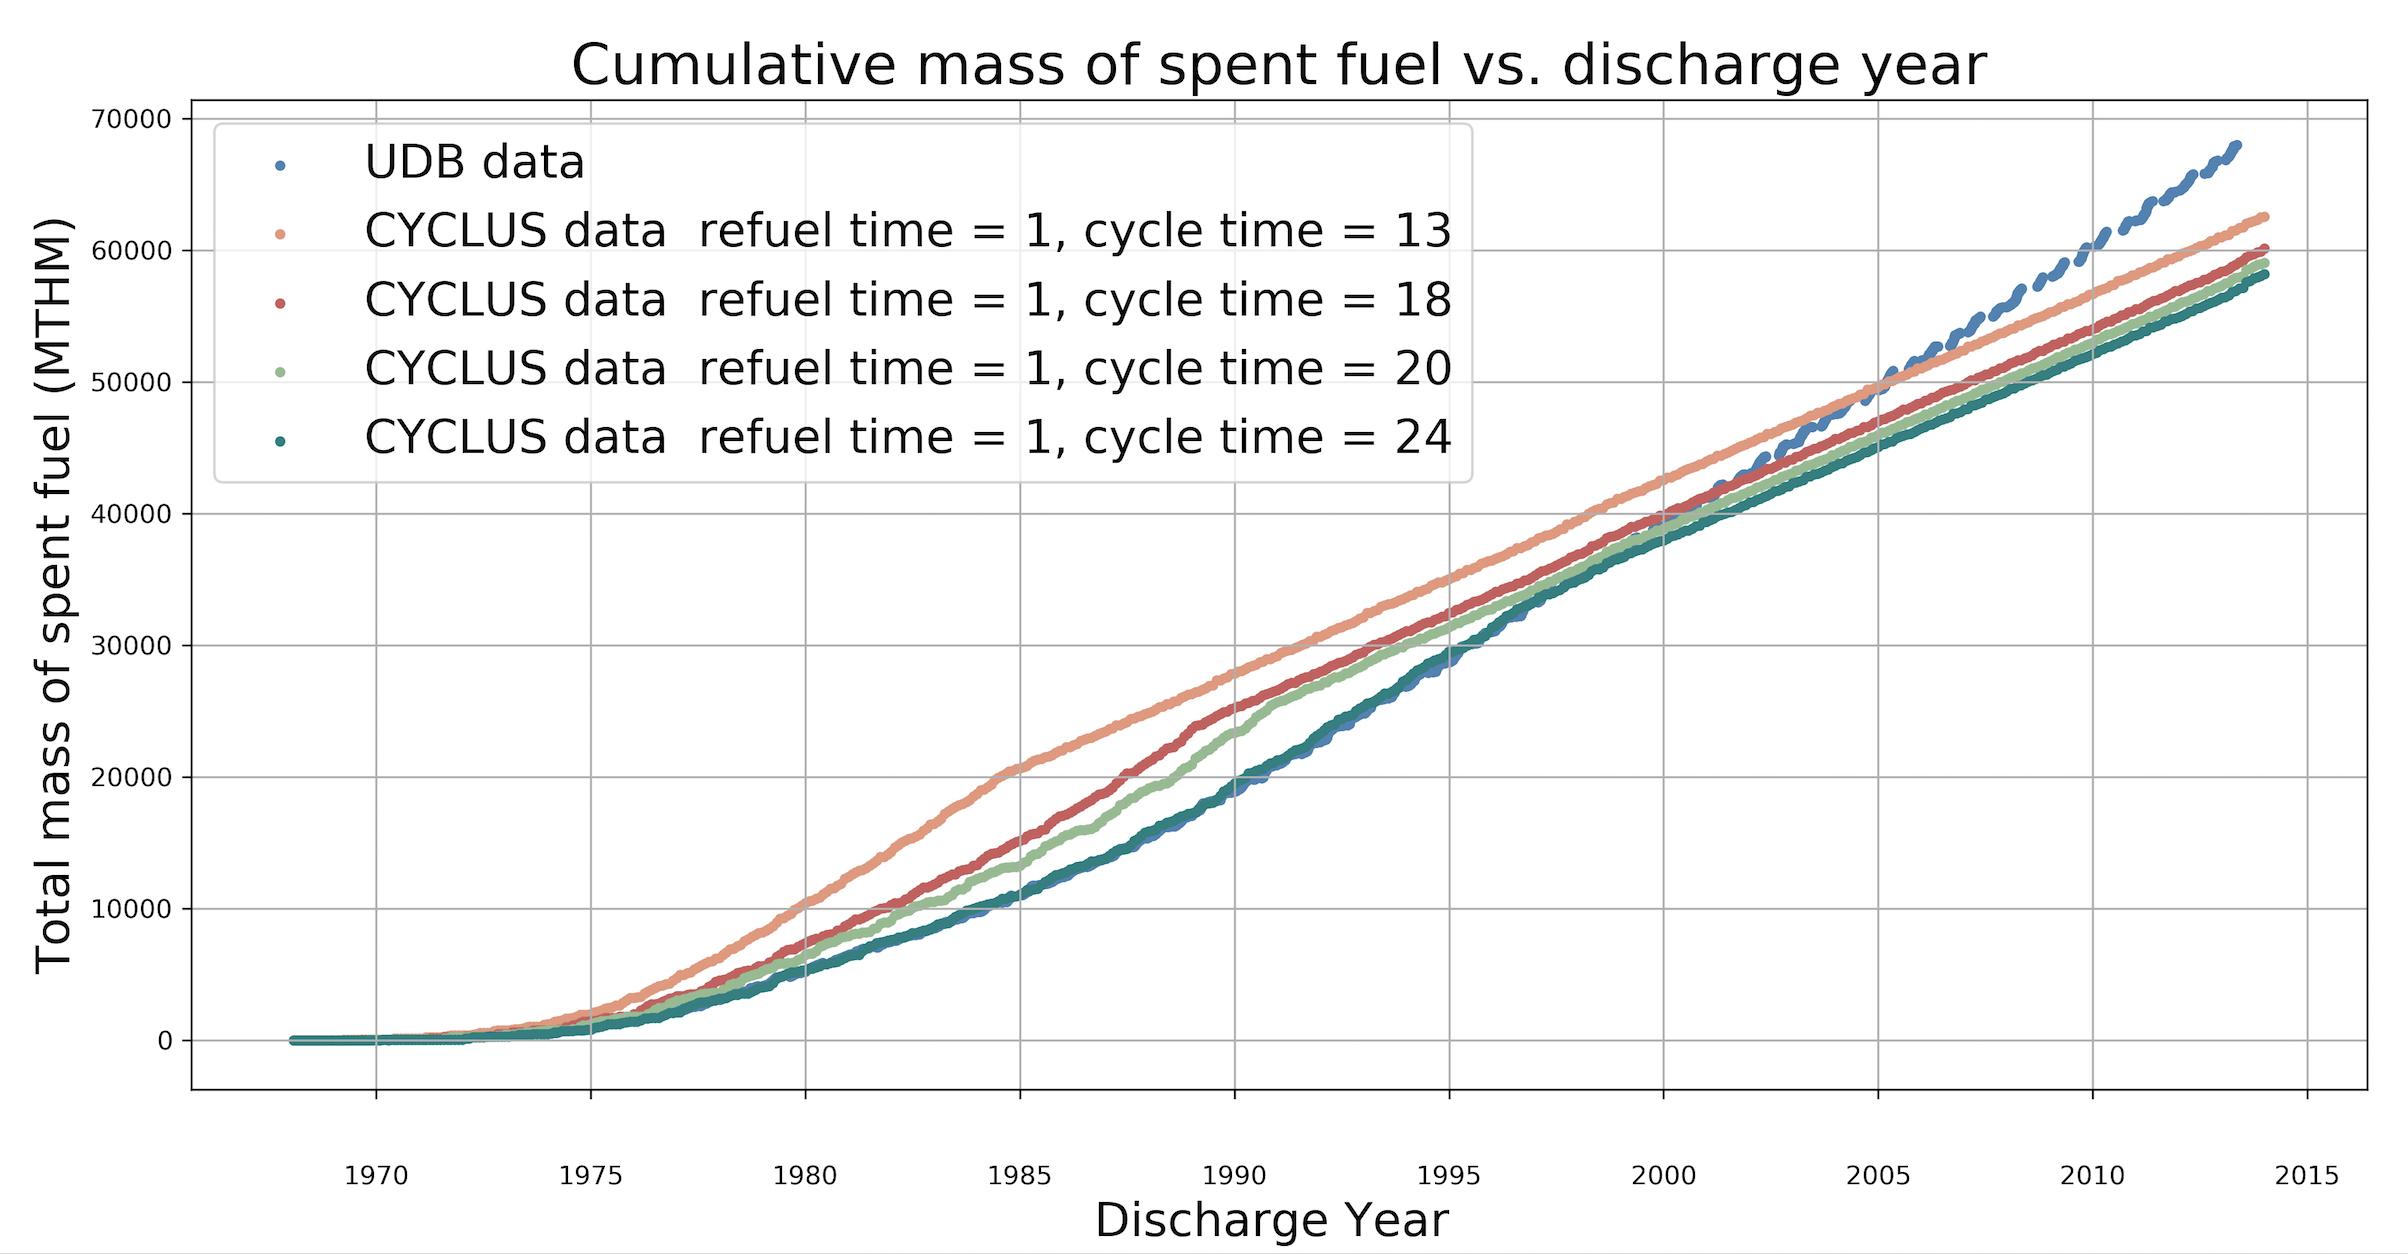
\includegraphics[width=0.48\textwidth]{total_cumulative_mass_spent_fuel_cycletime}
	\caption{Total cumulative spent fuel mass against discharge time for \Cyclus and UDB data from 1967 to 2013 for varying cycle time}
	\label{fig:total_cycletime}
\end{figure} 

\subsection{\textit{Major Isotopic Composition of  Spent Fuel Mass Comparison}}
The three isotopes that contribute the most to the total mass of the spent fuel in order of significance are: U-238, U-235, Pu-239.  

Figure \ref{fig:total_u238}, \ref{fig:total_u235} and \ref{fig:total_pu240} shows the cumulative spent fuel mass for U-238, U-235 and Pu-239 isotope for both \Cyclus and UDB data from 1967 to 2013.
They follow the same trend as figure \ref{fig:total_original} and the same explanations can be used to explain the differences in values. 

\begin{figure}[ht]
	\centering
	\begin{subfigure}[b]{0.45\textwidth}
		\centering
		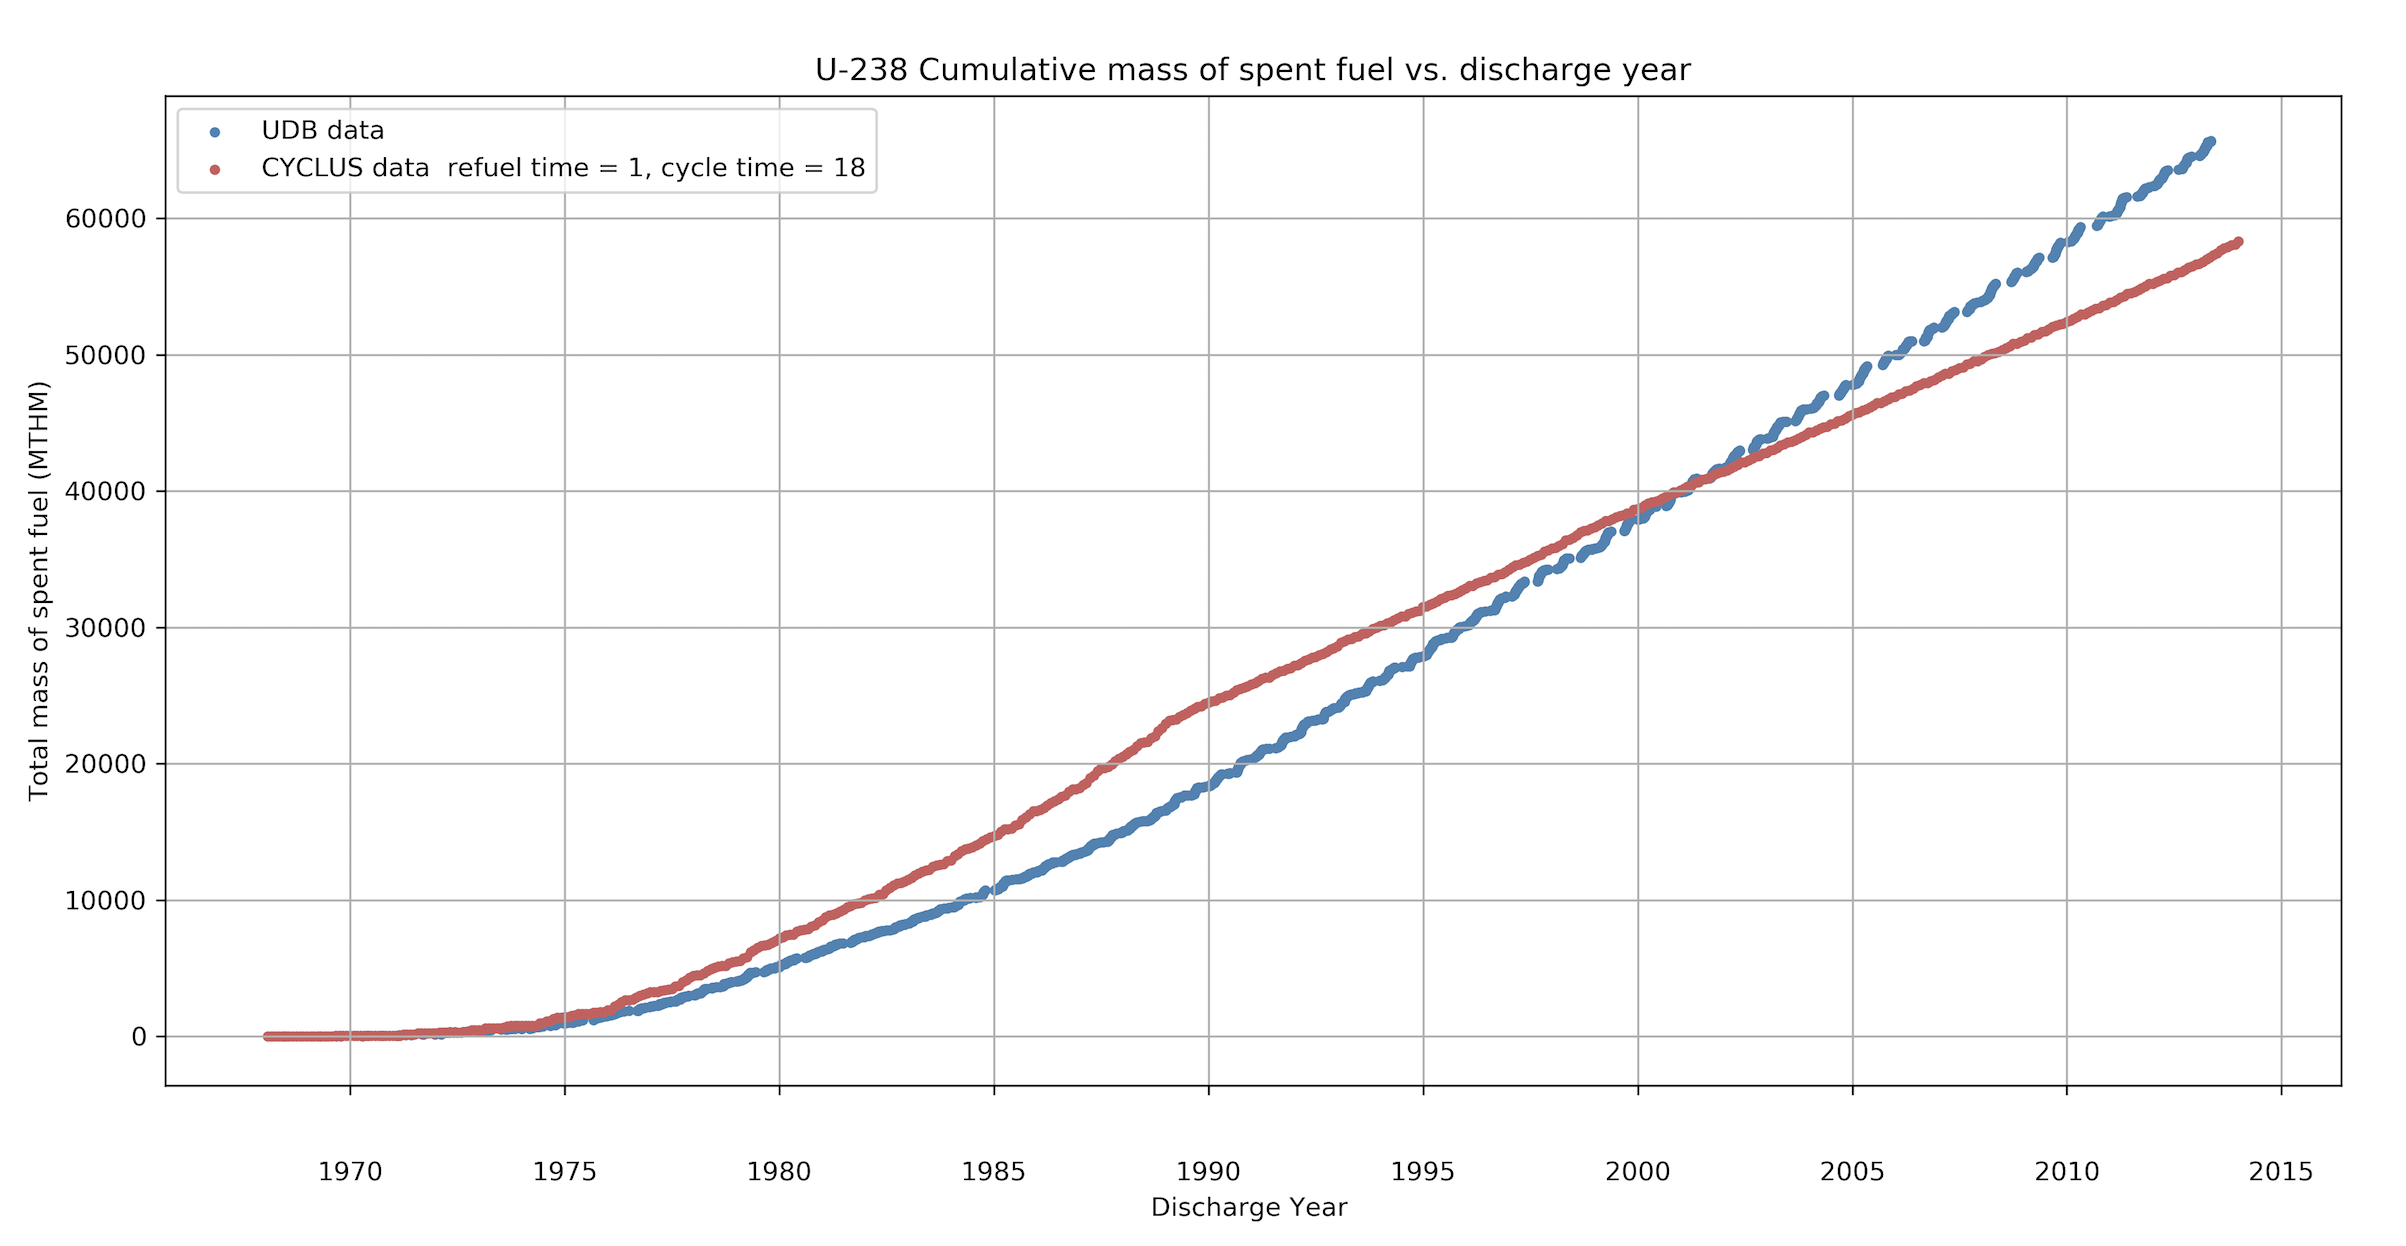
\includegraphics[width=\textwidth]{U-238_cumulative_mass_spent_fuel_original}
		\caption[Network2]%
		{{\small Timeseries of UOX waste produced}}    
		\label{fig:uoxwaste}
	\end{subfigure}
	\hfill
	\begin{subfigure}[b]{0.45\textwidth}  
		\centering 
		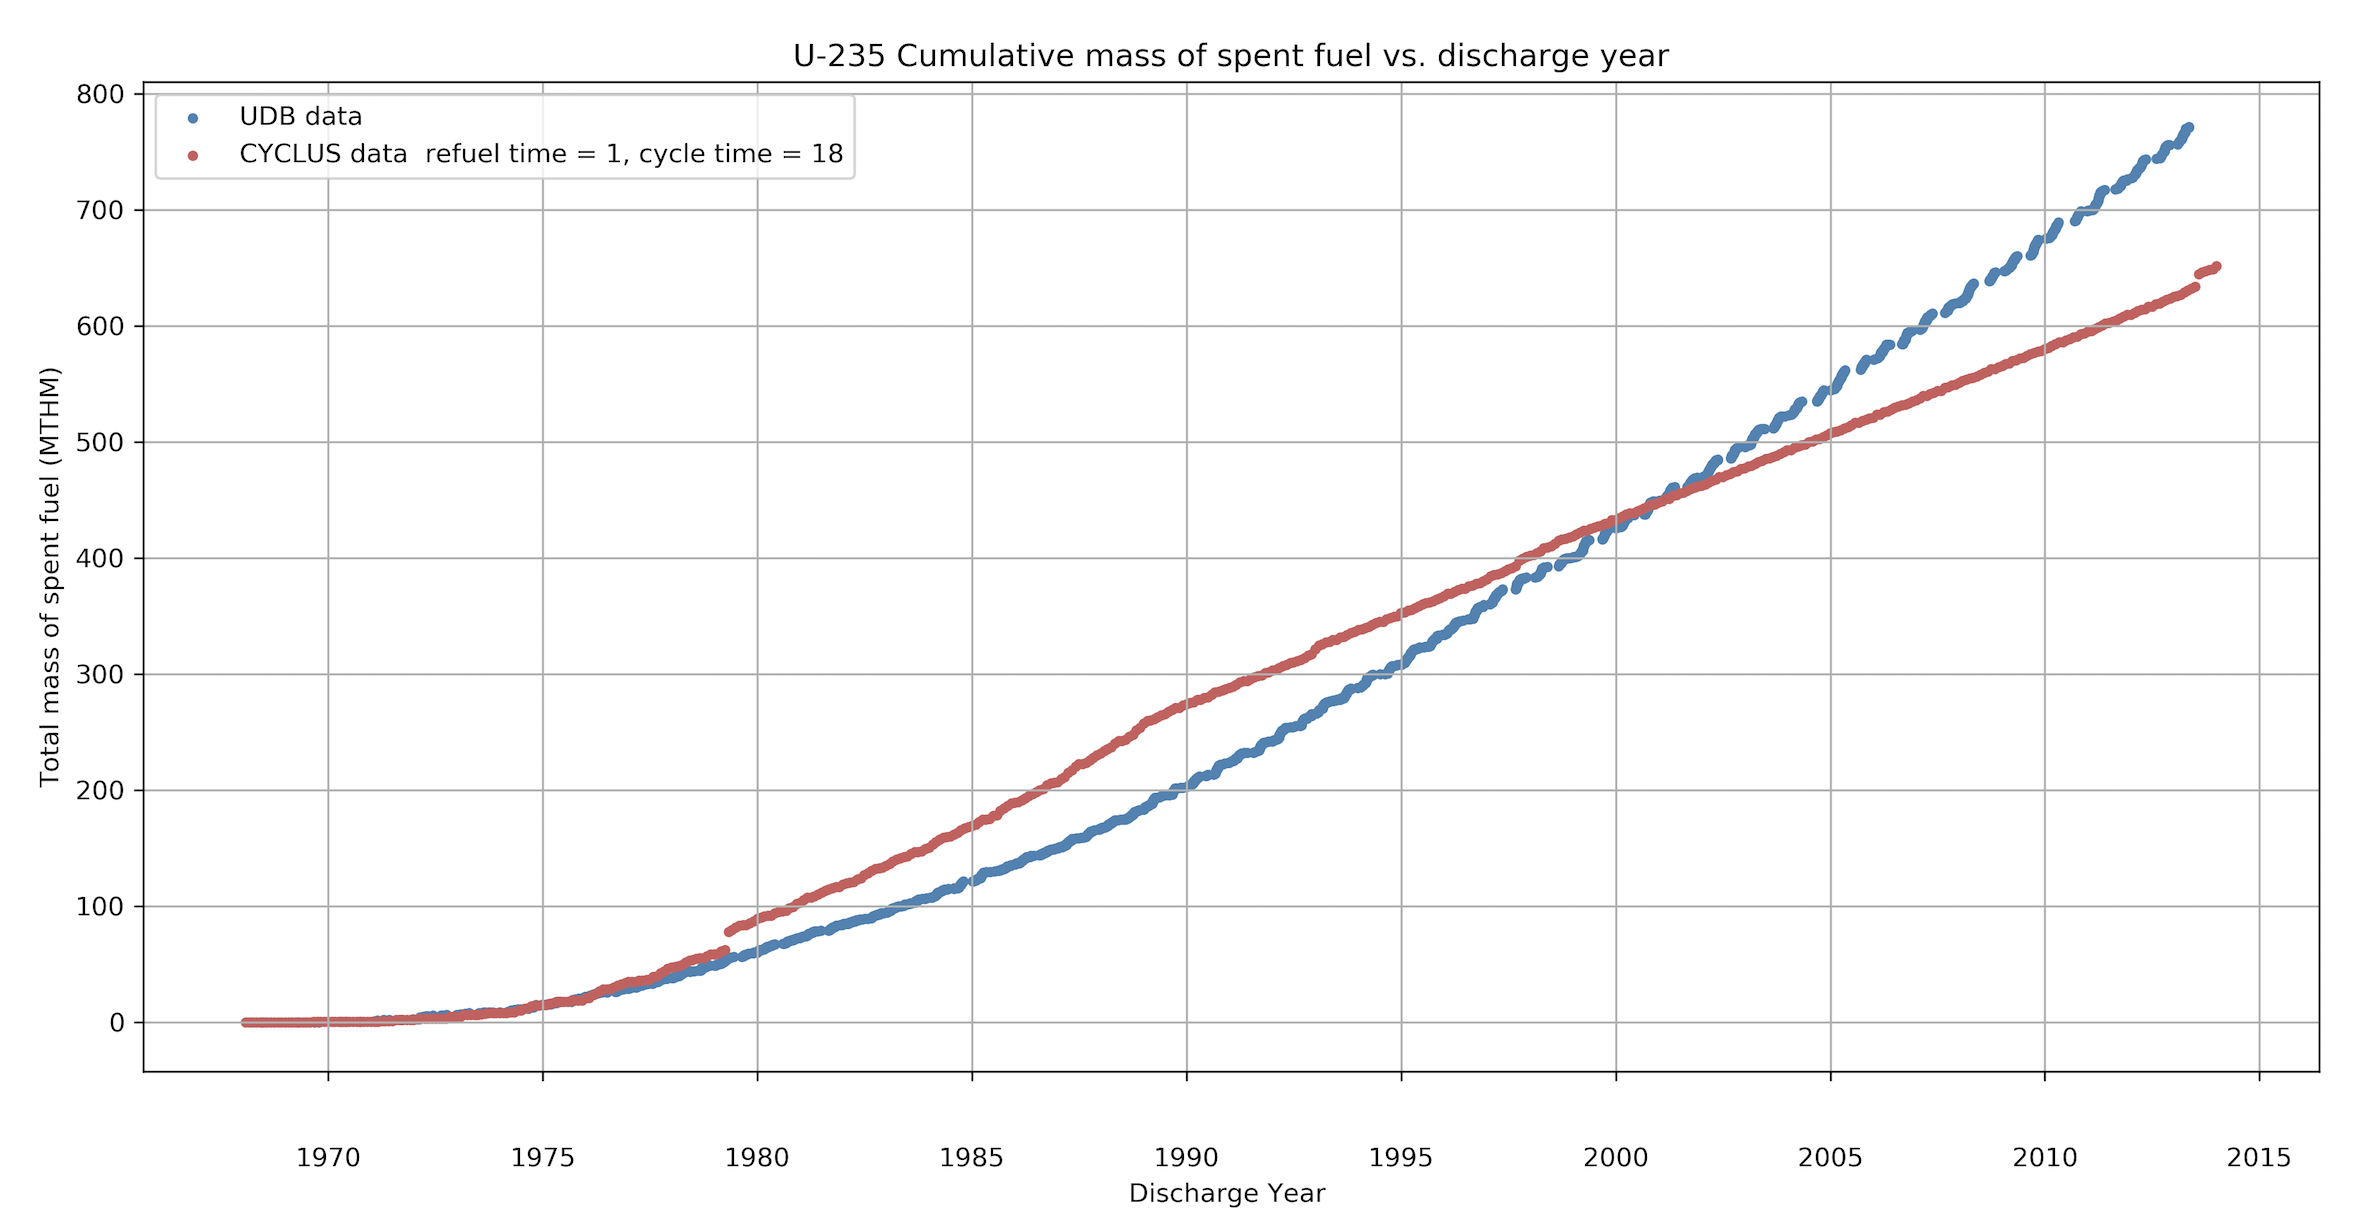
\includegraphics[width=\textwidth]{U-235_cumulative_mass_spent_fuel_original}
		\caption[]%
		{{\small Timeseries of Reprocess waste produced}}    
		\label{fig:reprocesswaste}
	\end{subfigure}
	\vskip\baselineskip
	\begin{subfigure}[b]{0.45\textwidth}   
		\centering 
		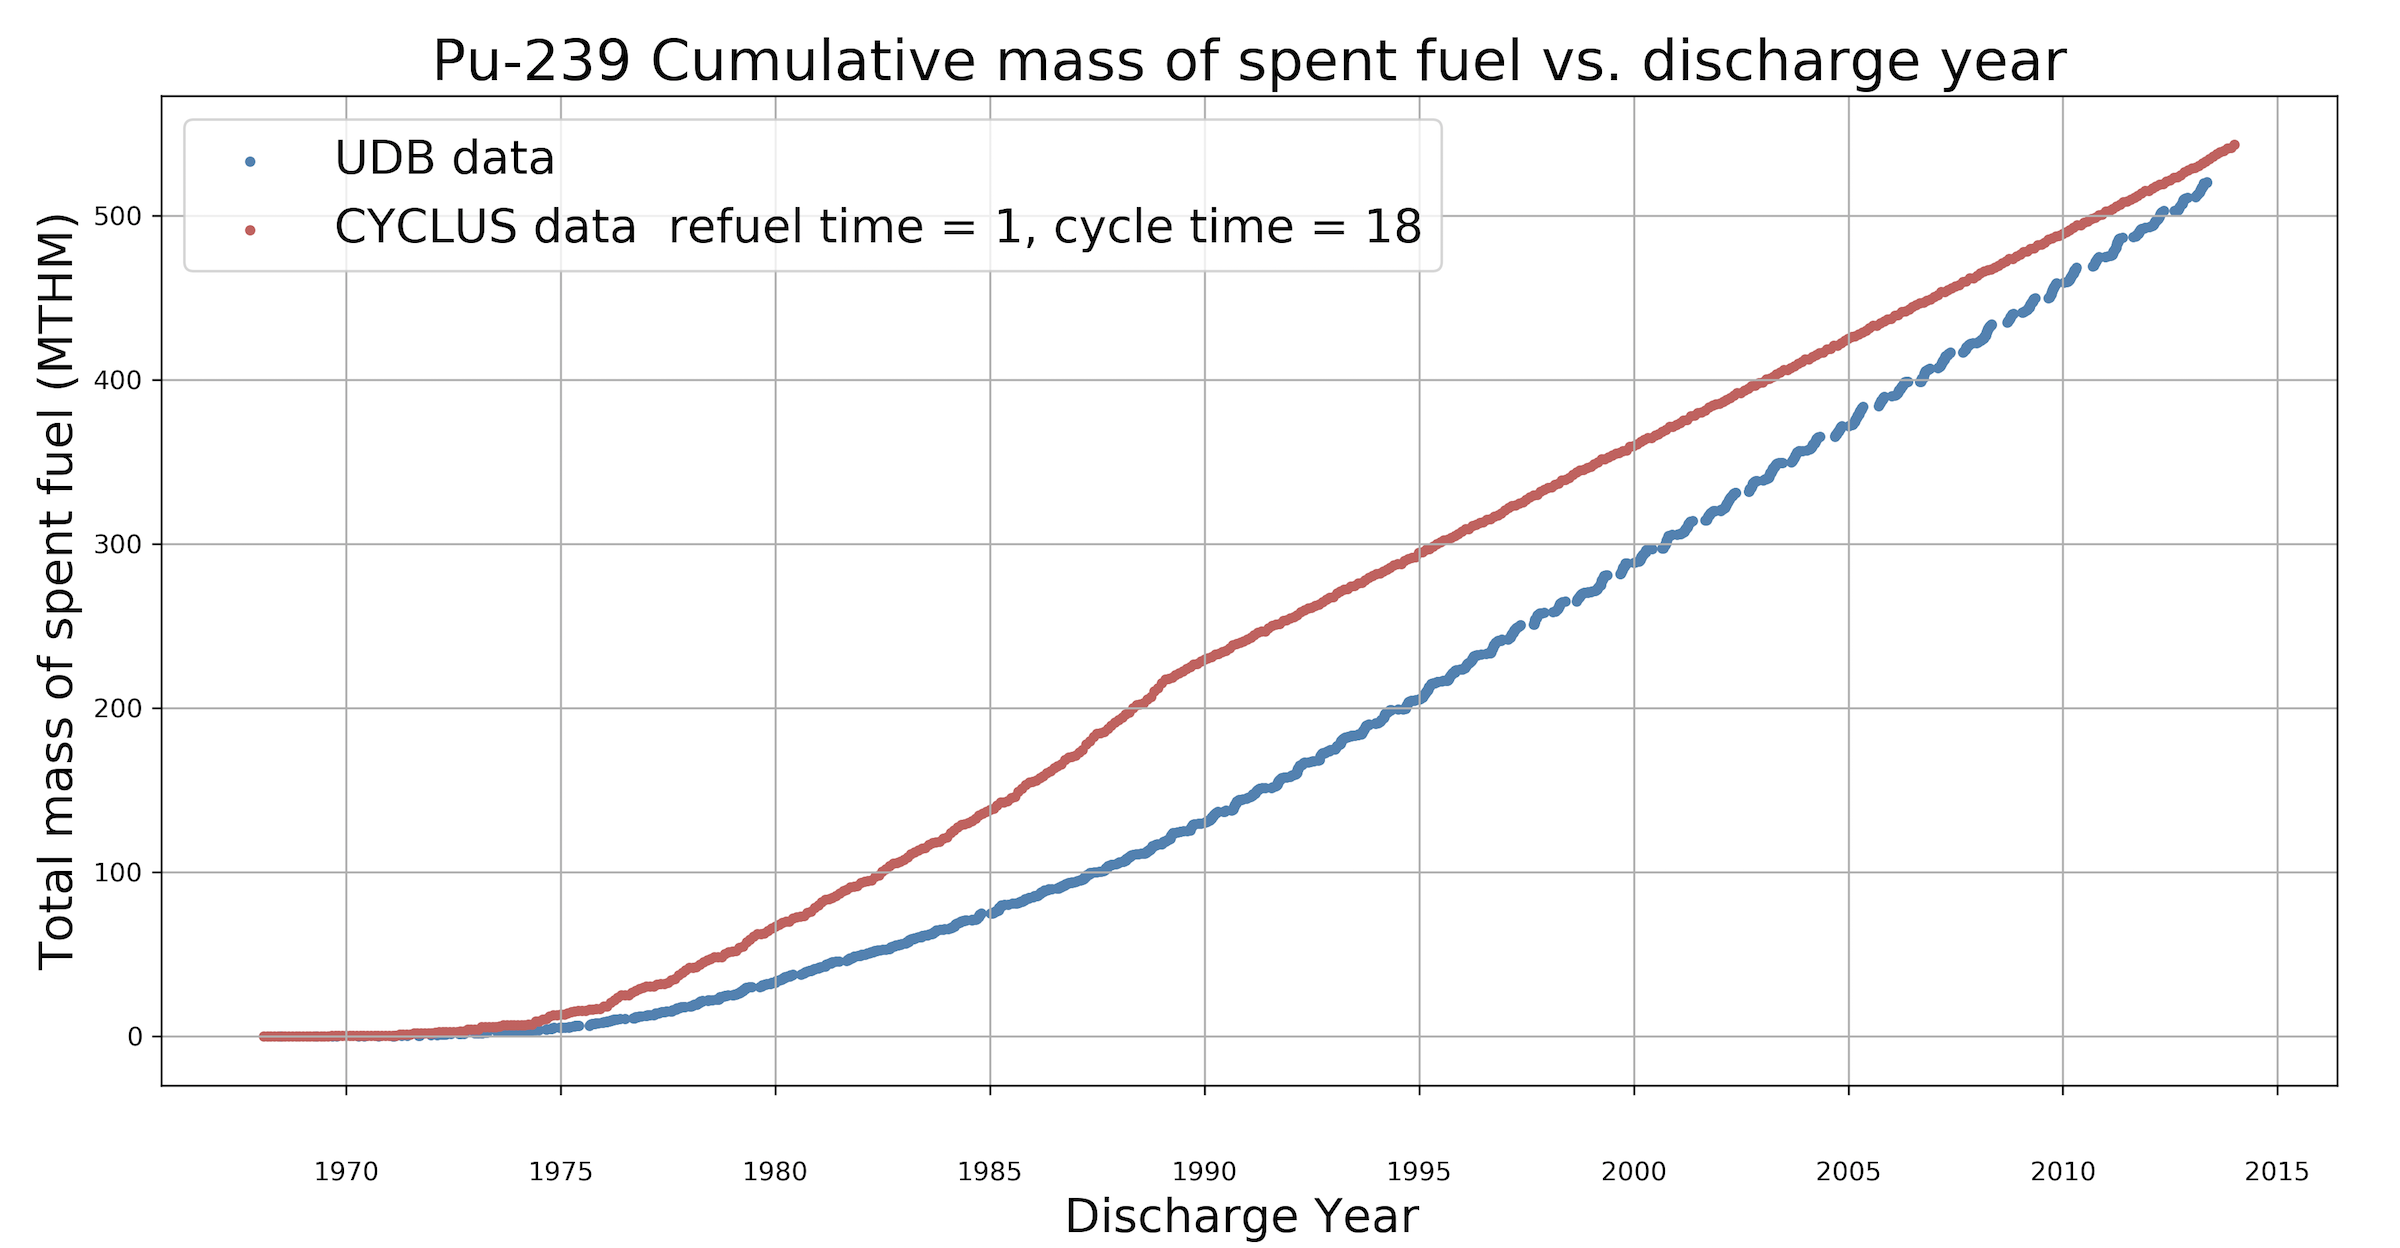
\includegraphics[width=\textwidth]{Pu-239_cumulative_mass_spent_fuel_original}
		\caption[]%
		{{\small Timeseries of UOX waste produced normalized for net capacity}}    
		\label{fig:normuoxwaste}
	\end{subfigure}
\end{figure}

%%%%%%%%%%%%%%%%%%%%%%%%%%%%%%%%%%%%%%%%%%%%%%%%%%%%%%%%%%%%%%%%%%%%%%%%%%%%%%%%
\section{Conclusions}
This work demonstrated that the spent fuel mass and isotopic composition results from the \Cyclus simulation of the United States nuclear fuel cycle closely follow the results from real world metrics. However, there is still improvements that can be made to replicate reality more closely. 

Further work that can help improve the simulation is to give the reactor archetype capability to accept varying cycle and refuel times. And so, by looking at the historic United States reactor operating data, a \Cyclus simulation can be made to replicate their cycle and refuel times even more closely. This would give more accurate spent fuel mass and isotopic compositions which will in turn make the simulations for thermal loading of a waste repository more accurate. 

%%%%%%%%%%%%%%%%%%%%%%%%%%%%%%%%%%%%%%%%%%%%%%%%%%%%%%%%%%%%%%%%%%%%%%%%%%%%%%%%
\section{Acknowledgments}
This research is being performed using funding received from the DOE Office of Nuclear Energy's
Nuclear Energy University Program (Project 16-10512) "Demand-Driven Cycamore Archetypes". 

%%%%%%%%%%%%%%%%%%%%%%%%%%%%%%%%%%%%%%%%%%%%%%%%%%%%%%%%%%%%%%%%%%%%%%%%%%%%%%%%
\bibliographystyle{ans}
\bibliography{bibliography}
\end{document}

